
\chapter{用于测试并发哈希表性能的框架——CHTBench}

\section{现有的测试方法比较}
\subsection{方法一}
方法描述:

优缺点:

\subsection{方法二}
方法描述:

优缺点:

\subsection{方法三}
方法描述:

优缺点:

\section{评估的指标选取}

\section{统一的跨平台并发哈希表测试框架的设计}
\label{sec:design_framework}

前文在进行并发哈希表介绍时提到,文献中提出的并发哈希表通常在设计(采用什么样的同步编程模型,基于锁还是无锁),实现(采用什么样的硬件优化方案)以及评估方法(总和的测试集合与测试方法)上都千差万别。
这些差异使得用户在横向上很难直观的进行比较,也很难判断究竟哪种因素限制了并发哈希表的性能。
在这部分内容里,将提出用于评估比较并发哈希表的测试框架CHTBench。
CHTBench能为参与评估的并发哈希表提供一个公平的测试环境,排除编译器、数据分布、线程调度方式、键值大小等因素的干扰。

\subsection{整体框架描述}

\subsection{资源管理}
% 包括线程、内存的管理。

\subsection{参数说明}
表~\ref{tab:concurrent_hash}列出的哈希表兼使用C/C++编写,为设计测试框架提供了便利。
可执行程序使用gcc 4.8编译生成,编译优化选项为'-O3'。
为了简便起见,所有的键值对均为64位整形数。
\textit{n}表示需要创建的线程数量,创建\textit{n}个线程用于并发的执行\textit{add},\textit{remove}和\textit{find}操作。
4个测试平台所能创建的最大线程数量见表~\ref{tab:arch_info}。
\textit{c}为范围在1到100的随机数,它用于控制执行查询和更新操作的比重,确保执行的操作的比重跟预期一致。
\textit{d}表示一次测试运行的时间,单位为毫秒,它用于控制\textit{while}循环什么时候结束。
创建的所有线程都将执行包含\textit{u}\%更新操作的工作集,\textit{u}表示更新操作占总的操作数量的百分比。
更新操作包含插入操作和删除操作,如没有特别说明,二者所占的比重是相同的。
因此,总的操作数中查询操作所占的比重为100 - \textit{u}\%。
\textit{i}为预先填充进哈希表的元素的个数,一般的\textit{i}为2的幂次方。
\textit{r}表示范围在1到2\textit{i}的值,它表示所产生的键的位置。
设置成最大值为2\textit{i}的目的是为了确保有50\%的操作是失败的操作。

\subsection{测试逻辑}
\label{sec:para_config}
多线程的创建和销毁都适用pthread库提供的接口。
在~\ref{sec:thread_pinning}~中详细介绍了三种不同的线程绑定方案,在测试文件有对应的核的排列方式。
编译时只需要输入相应的关键字就能使用对应的线程绑定方案进行编译。
哈希表的初始化在执行所有操作之前,初始化设置了两种方式,一是使用单个线程进行初始化;一是所有被创建的线程都参与初始化;
在使用多线程完成初始化时,每个线程获得均匀的初始化任务。
为了避免某些线程提前完成初始化转而执行其他操作,设置了内存屏障。
这样只有当所有的线程都完成了初始化任务,才会开始下一阶段的任务。

\begin{figure}[htbp]
\centering
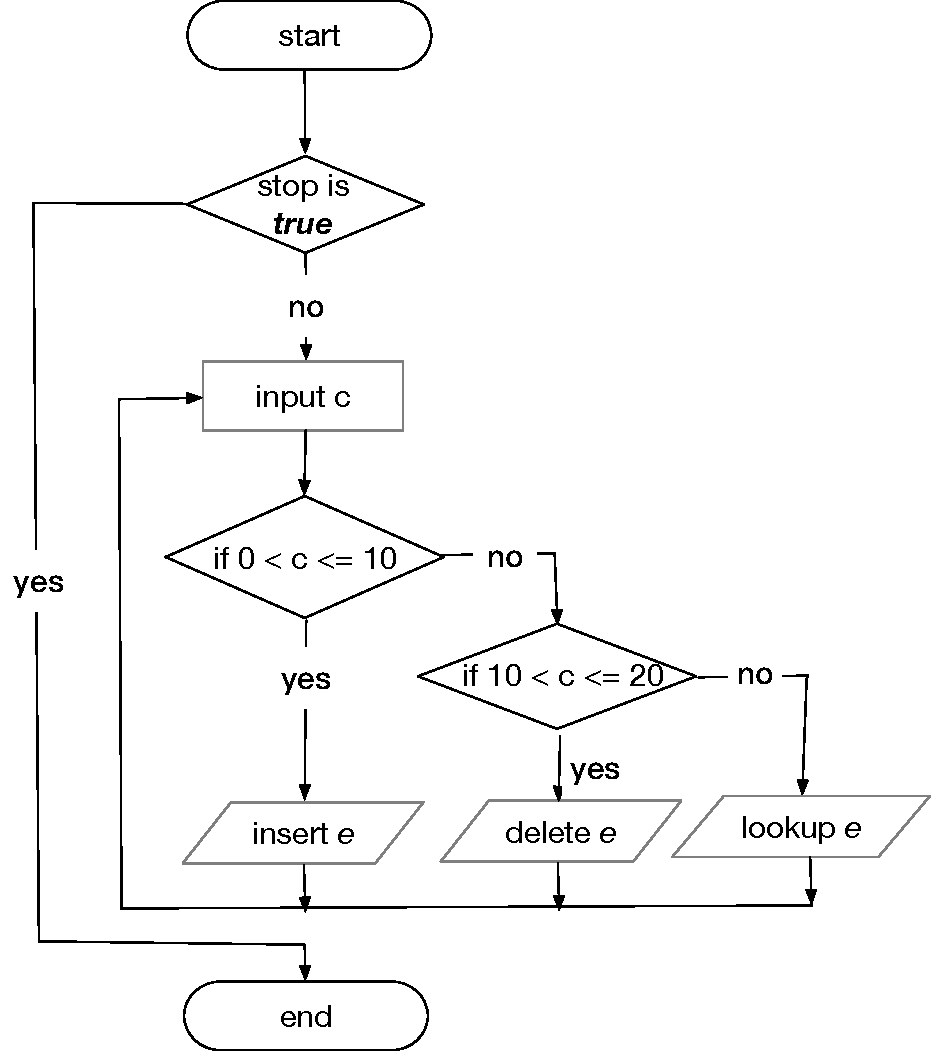
\includegraphics[width=0.9\textwidth]{flowchart_test}
\caption{CHTBench测试流程图}\label{fig:flowchart}
\end{figure}

如图~\ref{fig:flowchart}所示,
进入测试函数后,先判断此次执行哪种操作。
这个由随机值\textit{c}控制。
下面举例说明。
假设测试集中更新所占比重为20\%,则插入和删除各占10\%,而查询操作所占的比重为80\%,如果0 < \textit{c} <= 10时,执行插入操作;10< \textit{c} <= 20执行删除操作;而\textit{c}为其他值时则执行查询操作。

为了统计执行的总的操作次数,以及各项操作执行成功和失败的次数,每执行完一次操作,相应的计数器加1。最终通过统计相关计数器的值再除以执行时间得到吞吐量。

\section{本章小结}
